

\documentclass{beamer}
\beamertemplatenavigationsymbolsempty

\usepackage[utf8]{inputenc}         % Input encoding (allow direct use of special characters like "ä")
%\usepackage[english]{babel}
\usepackage[ngerman]{babel}
\usepackage[T1]{fontenc}
\usepackage[automark]{scrpage2} 	 % Schickerer Satzspiegel mit KOMA-Script
\usepackage{setspace}           	 % Allow the modification of the space between lines
\usepackage{caption}
\usepackage{tikz}

\captionsetup[figure]{labelformat=empty}

\usepackage{pdfpages}
% Um .eps Files einzubinden
\usepackage{epstopdf}



\setbeamercovered{transparent}
\beamertemplatenavigationsymbolsempty
\setbeamertemplate{footline}[frame number]

\usetheme{Madrid}

\AtBeginSection[]{
  \begin{frame}
  \vfill
  \centering
  \begin{beamercolorbox}[sep=8pt,center,shadow=true,rounded=true]{title}
    \usebeamerfont{title}\insertsectionhead\par%
  \end{beamercolorbox}
  \vfill
  \end{frame}
}


\title[Seminar]{Seminar e-Learning und Wissenskommunikation}
\subtitle[Remailer]{Adaptives Lernen}
\author[M. McCreight]{Mervyn McCreight}
\institute[FH-Wedel]{FH-Wedel}

\subject{Adaptives Lernen}
\keywords{Adaptives Lernen, Lernsoftware, Intelligente Tutorielle Systeme, Lernen, Lernparadigma}

\begin{document}

  \usetikzlibrary{positioning}
  \usetikzlibrary{shapes}
  \usetikzlibrary{arrows,automata}


\frame{\titlepage}

\begin{frame}
	\frametitle{Inhaltsverzeichnis}
	\tableofcontents
\end{frame}

\section{Einleitung}
\begin{frame}
  \frametitle{Aktuelles (1)}

  \begin{block}{Was wird mit Computerlernen verbunden?}
    \begin{itemize}
      \item klassische Lernsoftware
      \item fester Lernweg
      \item Wissensanzeige und -abfrage
      \item Vokabellernen
    \end{itemize}
  \end{block}

  \begin{block}{Diskussion (Stand 2014)}
    \begin{itemize}
      \item USA: Adaptive Lernsysteme für indiv. Betreuung in Schule
      \item GER: berufliche Aus-/Weiterbildung
    \end{itemize}
  \end{block}
\end{frame}

\begin{frame}
  \frametitle{Aktuelles (2)}

  \begin{block}{Horizon Report 2014}
    \begin{itemize}
      \item bescheinigt Lernassistenten (Tutoren) großes Potential
      \item hohe Weiterverbreitung in nächsten 4-5 Jahren an Hochschulen
    \end{itemize}
  \end{block}

  \begin{block}{INTUITEL}
    \begin{itemize}
      \item aktuelles Forschungsprojekt an Hochschule Karlsruhe
      \item klassische Lernsoftware mit tutoriellen Fähigkeiten anreichern
    \end{itemize}
  \end{block}
\end{frame}

\section{Adaptives Lernen in der Lerntheorie}
  \begin{frame}
    \frametitle{Bedeutung}
    \begin{block}{Bedeutung}
      Adaptives Lernen bedeutet, Lernangebote für den Unterricht zu finden, die Schüler trotz unterschiedlicher Voraussetzungen, gleichermaßen fördern.
    \end{block}

    \centering
    \begin{itemize}
      \item Anpassung der Lernumgebung
      \item Dynamischer Unterricht
      \item Individualität
    \end{itemize}
  \end{frame}
\subsection{Vergleich zum klassischen Lehrmodell}
  \begin{frame}
   \frametitle{Vergleich Lernparadigmen}
   \begin{block}{Vergleich Lernparadigmen}
      \begin{table}[!htbp]
        \centering
        \begin{tabular}{c || c | c}
          \hline
          \  & \textbf{Behaviorismus} & \textbf{Kognitivismus} \\
          \hline
          \textbf{Hirn ist} & passiver Behälter & Informationsverarbeitend \\
          \textbf{Wissen ist} & Input-Output Relation & interner Verarbeitungsprozess \\
          \textbf{Paradigma} & Stimulus-Response & Problemlösung  \\
          \textbf{Strategie} & Lehren & Beobachten und Helfen \\
          \textbf{Lehrer ist} & Autorität & Tutor \\
          \textbf{Interaktion} & starr & dynamisch, abhängig von Tutorand \\
        \end{tabular}
      \end{table}
   \end{block}
  \end{frame}

  \begin{frame}
  \frametitle{Vergleich Lernparadigmen}
    \begin{alertblock}{Behaviorismus}
     \begin{itemize}
       \item Alle lernen gleich
       \item statisch geplanter Unterricht
       \item Wissensreplikation
     \end{itemize}
    \end{alertblock}

    \begin{block}{Kognitivismus}
     \begin{itemize}
       \item Lernen ist individuell
       \item dynamisch angepasster Unterricht
       \item Problemlösung
     \end{itemize}
    \end{block}
  \end{frame}
\subsection{Aptitude-Treatment Interaktion}
\begin{frame}
  \frametitle{Aptitude-Treatment Interaktion}

  \begin{block}{Zweck}
    Forschung, um nachzuweisen, dass Lernen individuell ist
  \end{block}

  \begin{block}{deutsch:}
    Fähigkeits-Verfahrens-Wechselbeziehung
  \end{block}

  \begin{itemize}
    \item Grundfähigkeiten: Charakter, Vorwissen, Lerntyp
    \item Verfahren: Lehrmethoden, Lehrmittelpräsentation
    \item Führte zur Betrachtung von adaptivem Lernen
  \end{itemize}
\end{frame}
\subsection{Adaptionsmaßnahmen}
\begin{frame}
  \frametitle{Adaptionsmaßnahmen - Makroebene}
  \begin{block}{Makroebene}
    \begin{itemize}
      \item Maßnahmen auf Klassenebene
      \item Einteilung nach Leistungsniveau
      \item Angepasster Lehrplan für die Gruppen
    \end{itemize}
  \end{block}

  Beispiel: Altes Schulsystem - Hauptschule, Realschule, Gymnasium
\end{frame}

\begin{frame}
  \frametitle{Adaptionsmaßnahmen - Mikroebene}
  \begin{block}{Mikroebene}
    \begin{itemize}
      \item direkte Kommunikation
      \item Eingehen auf Stärken und Schwächen
      \item individuelle Anpassung der Lehrmethoden
      \item laufender Anpassungsprozess des Unterrichts
    \end{itemize}
  \end{block}

  Beispiele: Verschiedene Lerntypen - bildliche oder textliche Erklärung passt besser
\end{frame}

\subsection{Adaptionszwecke}
\begin{frame}
  \frametitle{Adaptionszwecke - Fördermodell}
  \begin{block}{Fördermodell}
    \begin{itemize}
      \item Beseitigung von Lerndefiziten
      \item Verständnis möglich, Wissen noch nicht erreicht.
      \item Zusatzaufgaben
      \item Schüler fördern, bis Lernziel erreichbar ist.
    \end{itemize}
  \end{block}
\end{frame}

\begin{frame}
  \frametitle{Adaptionszwecke - Kompensationsmodell}
  \begin{block}{Kompensationsmodell}
    \begin{itemize}
      \item Kompensation von Lerndefiziten
      \item Ausgleich unzureichender Lernvoraussetzungen
      \item schlechte Motivation, Überforderung
      \item individuelle Hilfestellungen - z.B. Betreuung, Nachhilfe
    \end{itemize}
  \end{block}
\end{frame}

\begin{frame}
  \frametitle{Adaptionszwecke - Präferenzmodell}
  \begin{block}{Präferenzmodell}
    \begin{itemize}
      \item Verwendung von individuellen Stärken und Schwächen
      \item besondere Voraussetzungen ausnutzen
      \item Anpassung der Aufgaben und des Unterrichts
      \item schnellerer Lernerfolg
    \end{itemize}
  \end{block}
\end{frame}

\section{Adaptives Lernen im e-Learning}
\begin{frame}
  \frametitle{Motivation}
    \begin{alertblock}{Bisher}
      \begin{itemize}
        \item behavioristische Lernsysteme
        \item menschliche Unterstützung
        \item nicht \glqq modern\grqq{} - Lernforschung
      \end{itemize}
    \end{alertblock}

    \begin{block}{Ziel}
      \begin{itemize}
        \item aktuelle Lernforschung berücksichtigen
        \item keine menschliche Unterstützung
        \item gleichwertig mit normalem Unterricht
      \end{itemize}
    \end{block}
\end{frame}

\begin{frame}
  \frametitle{Möglichkeiten}
  \begin{block}{Hypermediale Lernsysteme}
    \begin{itemize}
      \item Verbund von hypermedialen Wissenseinheiten
      \item freie, angepasste Navigation
      \item vielfältige Präsentationsauswahl
      \item entdeckendes Lernen
    \end{itemize}
  \end{block}

  \begin{block}{Intelligente Tutorielle Systeme}
    \begin{itemize}
      \item Erweiterung klassischer Lernsoftware
      \item Lehrverhalten angepasst an Lerner
      \item Tutor = Unterstützer
    \end{itemize}
  \end{block}
\end{frame}


\subsection{Intelligente Tutorielle Systeme}
\begin{frame}
  \frametitle{Intelligente Tutorielle Systeme}
  \begin{block}{Definition}
    Intelligente tutorielle Systeme (ITS) sind adaptive Mediensysteme, die sich ähnlich
    einem menschlichen Tutor an die kognitiven Prozesse des Lernenden anpassen
    sollen, indem sie die Lernfortschritte und -defizite analysieren und dementsprechend
    das Lernangebot generativ modifizieren sollen.
  \end{block}

  \begin{itemize}
    \item Adaptivität
    \item Adaptierbarkeit
  \end{itemize}
\end{frame}

\begin{frame}
  \frametitle{Grundanforderungen}
  \begin{block}{Adaptivität}
    \begin{itemize}
      \item Lehrplan und Geschwindigkeit, Aufgabentyp
      \item dynamisch während des Lernens
      \item System muss mitlernen -> Schüler
    \end{itemize}
  \end{block}

  \begin{block}{Flexibilität}
    \begin{itemize}
      \item Darstellung Lerninhalte
      \item angepasst an Lerner
    \end{itemize}
  \end{block}

  \begin{block}{Diagnosefähigkeit}
    \begin{itemize}
      \item Kernaspekt
      \item Analyse des Lernenden
      \item Wissensstand
      \item Stereotyp
    \end{itemize}
  \end{block}
\end{frame}
\subsection{Unterschied zu klassischen Lehrsystemen}
\begin{frame}
  \frametitle{Klassisches Lernsystem - Ablauf}

  \begin{figure}[!htb]
  	\centering
  	\begin{tikzpicture}[
  				part/.style={rectangle, minimum width=2cm, minimum height=1cm, very thick, draw=black, font=\itshape}
  				]
  		\node (start) [part] {Programmstart};
  		\node (presentation) [part, right=of start] {Lehrstoffpräsentation};
  		\node (question) [part, right=of presentation] {Fragestellung};
      \node (end) [part, below=of start] {Programmende};
      \node (feedback) [part, below=of presentation, right=of end] {Feedback};
  		\node (analyze) [part, below=of question, right=of feedback] {Analyse der Antwort};


  		\draw [->] (start) -- (presentation);
  		\draw [->] (presentation) -- (question);
  		\draw [->] (question) -- (analyze);
  		\draw [->] (analyze) -- (feedback);
  		\draw [->] (feedback) -- (presentation);
  		\draw [->] (feedback) -- (end);
  	\end{tikzpicture}

  	\caption{Prinzip eines klassischen tutoriellen Systems}
  \end{figure}

  \begin{itemize}
    \item starr vorgegebener Lehrplan
    \item richtig vs. falsch
    \item Wiederholung
  \end{itemize}
\end{frame}

\begin{frame}
    \frametitle{Beispiel}

    \begin{figure}[!htb]
    	\centering
        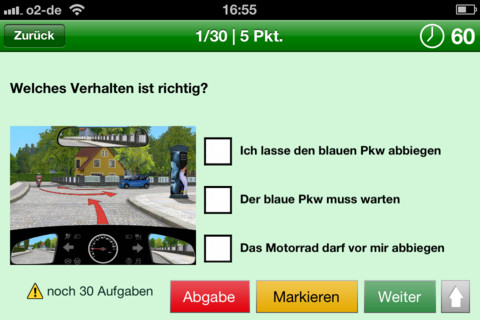
\includegraphics[width=0.7\textwidth]{../bilder/fahrschule_app.jpg} %70% der Textbreite
    	\caption{Beispielbild der Pocket Fahrschule Handy-Applikation}
    \end{figure}
\end{frame}

\begin{frame}
  \frametitle{Lernablauf - Intelligentes Tutorielles System}

  \begin{figure}[!htb]
  	\centering

  	\begin{tikzpicture}[->,>=stealth',
                      semithick]
  			\tikzstyle{comp2} = [fill=yellow, draw, rectangle, rounded corners, minimum height=0.8cm]
  			\tikzstyle{comp3} = [fill=black, text=white, draw, rectangle, rounded corners, minimum height=0.8cm]
  			\tikzstyle{comp1} = [draw, rectangle, rounded corners, minimum height=0.8cm]


        \node[comp1] (I) {Curriculum};
        \node[comp2] (A) [below=of I] {Erstelle Problem};
        \node[comp2] (B) [right=of A] {Präsentiere Problem};
        \node[comp2] (E) [right=of B] {Vergleiche Lösungen};
        \node[comp3] (C) [above=of E] {Student};
        \node[comp3] (D) [above left=of E] {Muster};
        \node[comp2] (F) [below=of E] {Analysiere Wissen};
        \node[comp2] (G) [left=of F] {Feedback};

  			\path (I) edge              (A)
  						(A) edge              (B)
  						(B) edge              (E)
  						(D) edge              (E)
  						(C) edge              (E)
  						(E) edge              (F)
  						(F) edge              (G)
  						(G) edge              (A);

  			\end{tikzpicture}
  \end{figure}

  \begin{columns}
    \begin{column}{0.5\textwidth}
       \begin{itemize}
         \item Feedback nach Wissensstand
         \item Lernproblem angepasst
       \end{itemize}
    \end{column}
    \begin{column}{0.5\textwidth}  %%<--- here
        \begin{itemize}
          \item flexibler Ablauf
          \item dauerhafte Re-Analyse
        \end{itemize}
    \end{column}
  \end{columns}
\end{frame}


\subsection{Architektur}
\begin{frame}
  \frametitle{Architektur}
    \begin{figure}[!htb]
    	\centering
        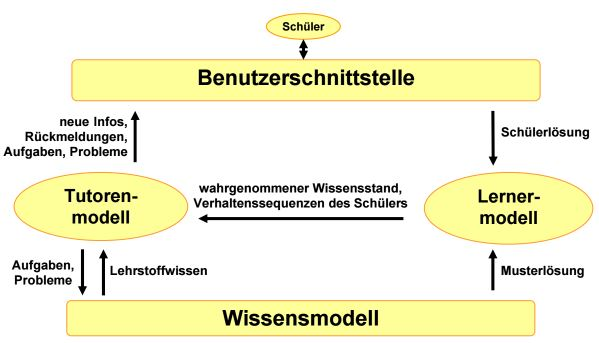
\includegraphics[width=0.7\textwidth]{../bilder/its_structure.jpg} %70% der Textbreite
    	\caption{Struktur eines Intelligenten Tutoriellen Systems}
    \end{figure}
\end{frame}

\begin{frame}
  \frametitle{Das Wissensmodell - Funktion}
  \begin{block}{Funktion}
    \begin{itemize}
      \item gesamtes Lehrwissen
      \item kommuniziert Lehrwissen für Aufgabenerstellung
      \item Musterlösungen für Bewertung
    \end{itemize}
  \end{block}
\end{frame}

\begin{frame}
  \frametitle{Das Wissensmodell - Wissensarten}
  \begin{block}{Deklaratives Wissen}
    \begin{itemize}
      \item Wissen-Was / Faktenwissen
      \item auswendig lernen
    \end{itemize}
  \end{block}

  \begin{block}{Prozedurales Wissen}
    \begin{itemize}
      \item Wissen-Wie / praktisches Wissen
      \item Regeln / Schemata
      \item Verständnis
      \item Verbindung von Faktenwissen
    \end{itemize}
  \end{block}

  \begin{block}{Heuristisches Wissen}
    \begin{itemize}
      \item Erfahrungswissen
      \item typische Fehler
      \item Handlungsempfehlungen / Tipps
    \end{itemize}
  \end{block}
\end{frame}

\begin{frame}
  \frametitle{Das Wissensmodell - Repräsentation}
  \begin{block}{Black-Box Modell}
    \begin{itemize}
      \item Lösungsweg verborgen
      \item unnatürliche Lösungsverfahren
      \item nur Lösung ist bekannt
      \item komplizierte Sachverhalte
    \end{itemize}
  \end{block}

  \begin{block}{Glass-Box Modell}
    \begin{itemize}
      \item Lösungsweg offen
      \item menschliche Lösungsverfahren
      \item Nachstellung menschlicher Intelligenz
      \item einfache Sachverhalte
      \item gezieltere Hilfestellung
    \end{itemize}
  \end{block}
\end{frame}

\begin{frame}
  \frametitle{Das Wissensmodell - Semantisches Netz}
  \begin{block}{Aufgaben}
    \begin{itemize}
      \item Sammlung von Wissenseinheiten
      \item Darstellung von Zusammenhängen
      \item Nützlich z.B. Voraussetzungsrelation
    \end{itemize}
  \end{block}
\end{frame}

\begin{frame}
  \frametitle{Das Wissensmodell - Semantisches Netz 2}
  \begin{figure}[!htb]
  	\centering

  	\begin{tikzpicture}[->,>=stealth', node distance=1.5cm and 1cm,
                      semithick]
  			\tikzstyle{comp2} = [fill=yellow, draw, rectangle, rounded corners, minimum height=0.8cm]

  			\node[comp2]	(A)                    	{Addition};
  			\node[comp2]  (B) [right=of A] 				{Subtraktion};
  			\node[comp2]  (C) [above=of A] 				{schriftl. Addition};
  			\node[comp2]  (D) [above of=B, right=of C] 	{schriftl. Subtraktion};
  			\node[comp2]  (E) [above of=A, left=of C] 	{Multiplikation};
  			\node[comp2]  (F) [above of=C] 	{Division};
  			\node[comp2]  (G) [above of=E] 	{schriftl. Multiplikation};

  			\path (A) edge              (B)
  						(A) edge              (C)
  						(A) edge              (E)
  						(B) edge              (D)
  						(C) edge              (D)
  						(E) edge              (G)
  						(E) edge              (F)
  			;
  			\end{tikzpicture}
  \end{figure}
\end{frame}

\begin{frame}
  \frametitle{Das Lernermodell}

  \begin{block}{Aufgabe}
    \begin{itemize}
      \item aktuell bekannter Wissensstand
      \item jede Aktion --> neue Bewertung
      \item auch: Historie der Aktionen
    \end{itemize}
  \end{block}

  \begin{block}{Wissensarten}
    \begin{itemize}
      \item deklaratives Wissen
      \item prozedurales Wissen
    \end{itemize}
  \end{block}

\end{frame}

\begin{frame}
  \frametitle{Das Lernermodell - Typisches Modell}
  \begin{block}{Overlay-Modell}
    \begin{itemize}
      \item Lernerwissen ist Teilmenge
      \item theoretisch: Wissen vs. Unwissen
      \item praktisch: Wissensgrad
      \item Fehler sind unvollständiges Wissen
    \end{itemize}
  \end{block}

  \begin{alertblock}{Nachteile}
    \begin{itemize}
      \item feststellbar: Wissen nicht vorhanden
      \item nicht feststellbar: teilweise falsch
      \item nicht feststellbar: korrektes Wissen falsch angewandt
    \end{itemize}
  \end{alertblock}
\end{frame}

\begin{frame}
  \frametitle{Das Lernermodell - Fehlerbibliothek}
  \begin{block}{Fehlerbibliothek}
    \begin{itemize}
      \item typische Fehler
      \item typische Missverständnisse
      \item Bsp: Vergessener Übertrag beim schriftl. Addieren
    \end{itemize}
  \end{block}

  \begin{alertblock}{Nachteile}
    \begin{itemize}
      \item häufig sehr groß
      \item unmöglich alle Fehler vorherzusehen
    \end{itemize}
  \end{alertblock}
\end{frame}

\begin{frame}
  \frametitle{Das Tutorenmodell}

  \begin{block}{Aufgaben}
    \begin{itemize}
      \item simuliert Verhalten eines Lehrers
      \item erhält Schülerinformation vom Lernermodell
      \item entscheidet über die Gestaltung und Ablauf des Unterrichts
    \end{itemize}
  \end{block}

  \begin{block}{Anforderungen}
    \begin{itemize}
      \item Passende Aufbereitung der Lehrstoffe
      \item Auswahl der Lehrstrategie
      \item Steuerung des Lehrtempos
      \item Wahl des aktuellen Lehrziels
    \end{itemize}
  \end{block}
\end{frame}

\begin{frame}
  \frametitle{Das Tutorenmodell - Lehrstandanalyse}
  \begin{block}{Deklaratives Wissen}
    \begin{itemize}
      \item Faktenwissen - richtig oder falsch
      \item leicht zu analysieren
      \item Maßnahmen - erneute Präsentation
    \end{itemize}
  \end{block}

  \begin{block}{Prozedurales Wissen}
    \begin{itemize}
      \item Regelwissen - falscher Lösungsweg oder Fehler im Lösunsweg?
      \item oft verschiedene richtige Lösungswege
      \item Model-Tracing
    \end{itemize}
  \end{block}

  \begin{block}{Model-Tracing Verfahren}
    \begin{itemize}
      \item korrekte Regeln bekannt
      \item Lösungswegebaum mit richtigen Lösungswegen
      \item Abweichung vom Baum = falsche Entscheidung
      \item Geraten oder gewusst?
    \end{itemize}
  \end{block}
\end{frame}

\begin{frame}
  \frametitle{Die Benutzerschnittstelle}

  \begin{block}{Aufgaben}
    \begin{itemize}
      \item Präsentation von Aufgaben, Feedback und Lehrstoff
      \item Navigation durch Benutzer
      \item Eingaben vom Benutzer entgegennehmen
    \end{itemize}
  \end{block}

  \begin{block}{Anforderungen}
    \begin{itemize}
      \item intuitiv bedienbar
      \item übersichtlich
      \item optimal: anpassbar
    \end{itemize}
  \end{block}

  \begin{block}{Möglichkeiten}
    \begin{itemize}
      \item textuell - Terminal mit Dialog
      \item Menüsystem - GUI
    \end{itemize}
  \end{block}
\end{frame}

\subsection{Möglichkeiten zur Umsetzung von Adaption}
\begin{frame}
  \frametitle{Adaptionsmöglichkeiten in ITS}
  \begin{block}{Sequenzierung}
    \begin{itemize}
      \item Anpassung der Reihenfolge
      \item Lernthemen und Wissenseinheiten
      \item vollständige Entfernung möglich
      \item Ziel: keine unnötigen Themen, keine unschaffbaren Fragen
    \end{itemize}
  \end{block}

  \begin{block}{Unterstützung}
    \begin{itemize}
      \item Anpassung der Lerngeschwindigkeit
      \item großschrittig vs. kleinschrittig
      \item Zusatzinformationen (auch zu anderen Themen, falls wichtig)
      \item Ziel: bewusste Themen schnell, schwere langsamer
    \end{itemize}
  \end{block}
\end{frame}

\begin{frame}
  \frametitle{Adaptionsmöglichkeiten in ITS (2)}

  \begin{block}{Adaptive Präsentation}
    \begin{itemize}
      \item Anpassung der Darstellungsart
      \item Lernstereotypen
      \item Ziel: Präsentation nutzt individuelle Stärken aus
    \end{itemize}
  \end{block}

  \begin{block}{Adaptive Navigation}
    \begin{itemize}
      \item Anpassung der Navigationsmöglichkeiten
      \item angepasst an Wissensstand
      \item Unmögliches filtern
      \item Ziel: optimaler Lernweg durch das Programm
    \end{itemize}
  \end{block}
\end{frame}

\section{Beispiel}
\subsection{Algebraland}
\begin{frame}
  \frametitle{Beispiel - Algebraland}
  \begin{block}{Beschreibung}
    \begin{itemize}
      \item Lösung von Gleichungen mit einer Unbekannten
      \item wenig Faktenwissen, viel Regelwissen
      \item Aufteilung: Lösungsweg planen und Planung umsetzen
    \end{itemize}
  \end{block}
\end{frame}

\begin{frame}
  \frametitle{Beispiel - Algebraland (2)}
  \begin{figure}
    \centering
    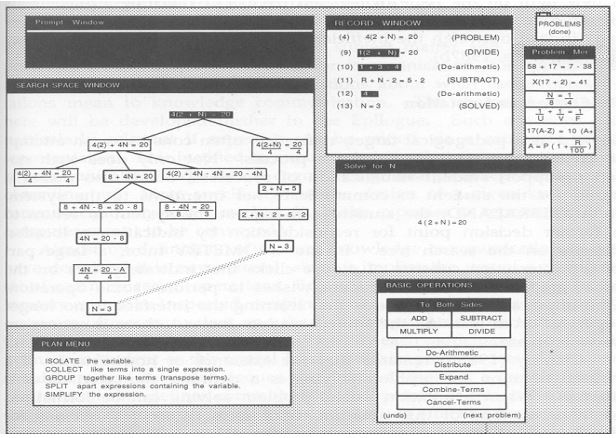
\includegraphics[width=0.7\textwidth]{../bilder/algebraland.jpg}
  \end{figure}

  \begin{itemize}
    \item Lösungswege Baumdiagramm
    \item Typisches Lernproblem mit vielen richtigen Lösungswegen
    \item Hilfe bei falschen Lösungsansätzen
  \end{itemize}

\end{frame}

\subsection{BRIDGE-Tutor}
\begin{frame}
  \frametitle{Beispiel - BRIDGE}
  \begin{block}{Beschreibung}
    \begin{itemize}
      \item Programmieren in Pascal
      \item Aufteilung in Strukturierung und Umsetzung
      \item Struktur sprachlich in Pseudocode
      \item später Umsetzung des Pseudocodes in Pascal
    \end{itemize}
  \end{block}
\end{frame}

\begin{frame}
  \frametitle{Beispiel - BRIDGE (2)}
  \begin{figure}
    \centering
    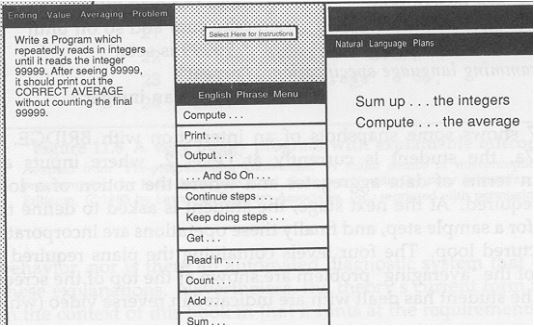
\includegraphics[width=0.7\textwidth]{../bilder/bridge1.jpg}
  \end{figure}

  \begin{itemize}
    \item natürlich sprachliche Strukturierung
    \item Verfeinerung Schritt für Schritt
    \item Jederzeit Hilfe anfordern
  \end{itemize}
\end{frame}

\begin{frame}
    \frametitle{Beispiel - BRIDGE(3)}
    \begin{figure}
      \centering
      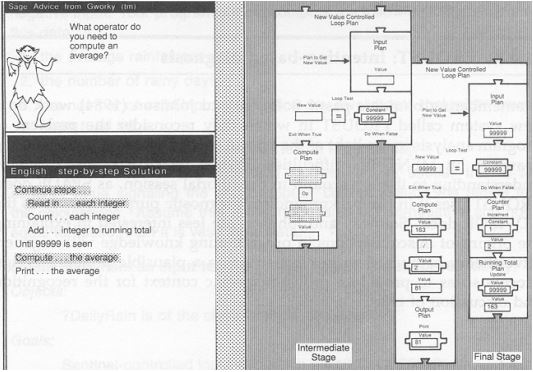
\includegraphics[width=0.7\textwidth]{../bilder/bridge2.jpg}
    \end{figure}
\end{frame}

\subsection{LISP-Tutor}
\begin{frame}
  \frametitle{Beispiel - LISP-Tutor}
  \begin{block}{Beschreibung}
    \begin{itemize}
      \item Programmieren in LISP
      \item Kommandozeile
      \item dynamisches Lehrgespräch (simulierter Dialog)
    \end{itemize}
  \end{block}

  \begin{figure}
    \centering
    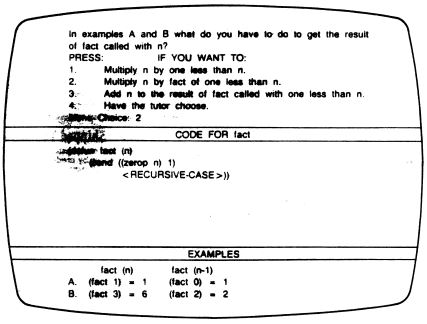
\includegraphics[width=0.5\textwidth]{../bilder/greaterp2.jpg}
  \end{figure}
\end{frame}

\begin{frame}
  \frametitle{Beispiel - LISP-Tutor (2)}
  \begin{alertblock}{Tutor}
    Define the function fact. It takes a number argument n, and computes the
    factorial of n, which is the result of multiplying n*(n-1)*(n-2) ... * 1.
    By definition, 0! is 1.
  \end{alertblock}

  \begin{block}{User}
    (defun fact(n)
      (cond ((equal) < ACTION >)
      <RECURSIVECASE>
    ))
  \end{block}

  \begin{alertblock}{Tutor}
    I assume that you are trying to test if the number argument is equal to
    the number zero. There is a special function for testing equivalence to zero.
    Try to use that function instead of equal.

    What code can you write to test if the condition for terminating case is true?
    Try writing a predicate!
  \end{alertblock}

\end{frame}

\begin{frame}
  \frametitle{Beispiel - LISP-Tutor(3)}
  \begin{alertblock}{Tutor}
    Is the value of fact in the recursive cases calculated by:\\
    PRESS:      IF YOU WANT TO:\\
    1           Calling fact recursively with n.\\
    2           Multiplying n by fact of n minus 1.\\
    3           Getting 1 2 ... n and then multiplying the results.\\
    4           Have the tutor choose.\\
  \end{alertblock}

  \begin{block}{User}
    3
  \end{block}

  \begin{alertblock}{Tutor}
    That is a reasonable way to think of doing factorials, but it is not a plan for a recursive function.
    Since you seem to be having trouble with the recursive cases, let us work through some examples and
    figure out the conditions and actions for each of these cases.
    (...)
  \end{alertblock}

\end{frame}



\section{Fazit}

\end{document}
